%-------------------------------------------------------------------------------
%                                PREAMBLE
%-------------------------------------------------------------------------------
\documentclass[usenames,dvipsnames,svgnames,10pt,aspectratio=169]{beamer}
\usefonttheme{professionalfonts}

% This theme uses TIKZ: compile twice with PDFLaTeX or LuaLaTeX.
%
%  Options:
%  - [clean]:    clean slides, i.e. logos and footbar are removed
%  - [kth]:      footbar style inspierd to the official KTH template
%  - [nicewave]: a different style of wave is used (not approved by FLOW)
%
\usetheme{flow}

\usepackage{hyperref,graphicx,lmodern}
\usepackage[utf8]{inputenc}
\usepackage{media9}
\usepackage{xcolor}
\usepackage{stmaryrd}
\usepackage{nicefrac}
\usepackage{multimedia}
\usepackage{multicol}
\usepackage{upgreek}
\usepackage[]{bm}
\usepackage[]{url}

\DeclareMathOperator{\sinc}{sinc}
\DeclareMathAlphabet{\mathcal}{OMS}{cmsy}{m}{n}
\DeclareMathAlphabet\mathbfcal{OMS}{cmsy}{b}{n}

\graphicspath{{imgs/}}
\setbeamertemplate{blocks}[rounded][shadow=true]

\DeclareMathOperator{\trace}{tr}

%-------------------------------------------------------------------------------
%                                TITLE PAGE
%-------------------------------------------------------------------------------
\title[Nonlinear Physics] % Short title used in footline
{
	Nonlinear physics, dynamical \\ systems and chaos theory
}

\author[J.-Ch.~Loiseau] % Presenting author in short form used in footline
{
	Jean-Christophe Loiseau
}
% - Give the names in the same order as the appear in the paper.
% - Underline the presenting author.

\institute[unused]
{
	\url{jean-christophe.loiseau@ensam.eu} \\
	DynFluid, \\
	Arts et M\'etiers ParisTech, France
}
% Keep it simple, no one is interested in your street address.

% University logo(s)
\logot{
\includegraphics[width=.128\paperwidth]{DynFluid_logo}}  % Top logo
\logob{
\includegraphics[width=0.128\paperwidth]{ENSAM_logo}} % Bottom logo
% \logoc[{
\includegraphics[width=.128\paperwidth]{limsi}}]{
\includegraphics[width=.128\paperwidth]{limsi}} % Corner logo
%
% Cover image: \cvrimg{x position}{y position}{cover image}
\cvrimg{.77}{.8}{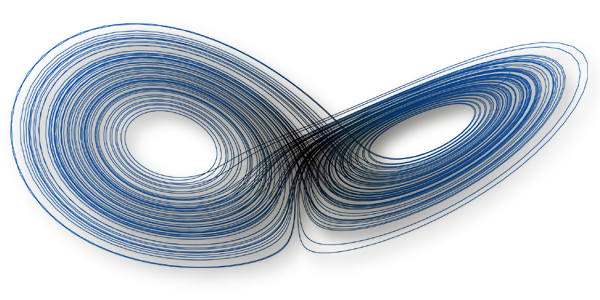
\includegraphics[width=.4\paperwidth]{cover.png}}

\date[unused]{ENSAM, Master 2, 2017--2018}

\begin{document}

\titleframe % Print the title as the first slide

%-------------------------------------------------------------------------------
%                           PRESENTATION SLIDES
%-------------------------------------------------------------------------------

\begin{frame}[t, c]{Today's menu}{Subharmonic cascade}
	\begin{itemize}
		\item So far, we have seen at least two sequences of bifurcations that cause a system to exhibit chaotic dynamics.
		\begin{itemize}
			\item[$\hookrightarrow$] \alert{\textbf{Logistic map}}: Sequence of period doubling bifurcations.
			\item[$\hookrightarrow$] \alert{\textbf{Lorenz system}}: For $0 \leq \rho \leq 25$, a supercritical pitchfork and a subcritical Hopf bifurcations occur before the creation of a stange attractor.
		\end{itemize}

		\bigskip

		\item These are two different routes to chaos. They are not the only ones though...

		\bigskip

		\item Today, we will focus exclusively on the sequence of period-doubling bifurcations
	\end{itemize}

	\vspace{1cm}
\end{frame}

\begin{frame}[t, c]{}
	\centering
	\vspace{1cm}

	{\Large \textbf{Logistic map}}

	\bigskip

	{\textgre{\textbf{A simple discrete-time model of population dynamics}}}

\end{frame}

\begin{frame}[t, c]{Logistic map}{A simple example}
	\begin{itemize}
		\item Let us consider once again the logistic map given by
		$$x_{k+1} = \mu x_k ( 1 - x_k),$$
		where $\mu$ is our control parameters.

		\bigskip

		\item We have studied this discrete-time system during Lecture 5.
	\end{itemize}

	\vspace{1cm}
\end{frame}

\begin{frame}[t, c]{Logistic map}{Cobweb and phase plane for $\mu = 1$}
	\begin{minipage}{.48\textwidth}
		\centering
		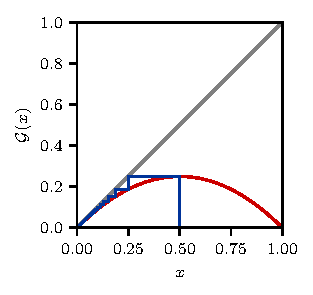
\includegraphics[width=.75\textwidth]{logistic_map_cobweb_plot_0}
	\end{minipage}%
	\begin{minipage}{.48\textwidth}
		\centering
		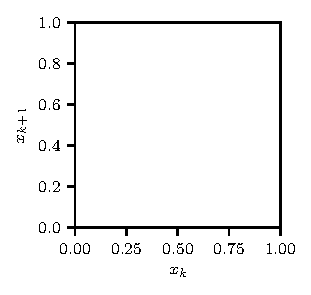
\includegraphics[width=.75\textwidth]{logistic_map_phase_plane_0}
	\end{minipage}

	\vspace{1cm}
\end{frame}

\begin{frame}[t, c]{Logistic map}{Cobweb and phase plane for $\mu = 1.32$}
	\begin{minipage}{.48\textwidth}
		\centering
		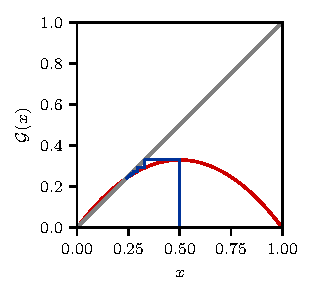
\includegraphics[width=.75\textwidth]{logistic_map_cobweb_plot_1}
	\end{minipage}%
	\begin{minipage}{.48\textwidth}
		\centering
		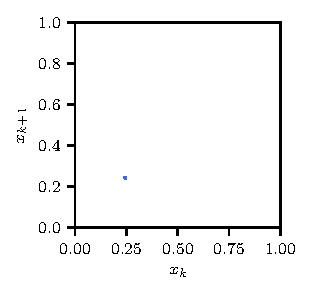
\includegraphics[width=.75\textwidth]{logistic_map_phase_plane_1}
	\end{minipage}

	\vspace{1cm}
\end{frame}

\begin{frame}[t, c]{Logistic map}{Cobweb and phase plane for $\mu = 1.64$}
	\begin{minipage}{.48\textwidth}
		\centering
		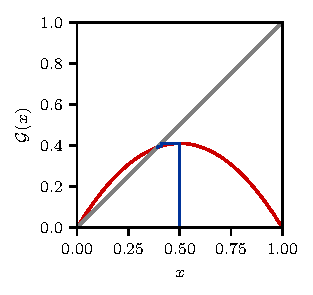
\includegraphics[width=.75\textwidth]{logistic_map_cobweb_plot_2}
	\end{minipage}%
	\begin{minipage}{.48\textwidth}
		\centering
		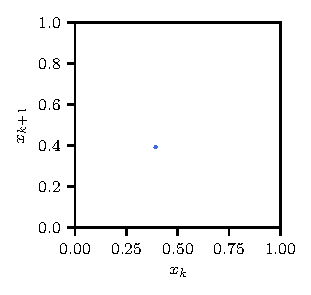
\includegraphics[width=.75\textwidth]{logistic_map_phase_plane_2}
	\end{minipage}

	\vspace{1cm}
\end{frame}

\begin{frame}[t, c]{Logistic map}{Cobweb and phase plane for $\mu = 1.96$}
	\begin{minipage}{.48\textwidth}
		\centering
		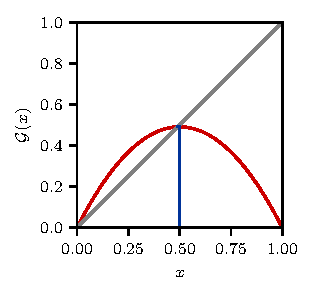
\includegraphics[width=.75\textwidth]{logistic_map_cobweb_plot_3}
	\end{minipage}%
	\begin{minipage}{.48\textwidth}
		\centering
		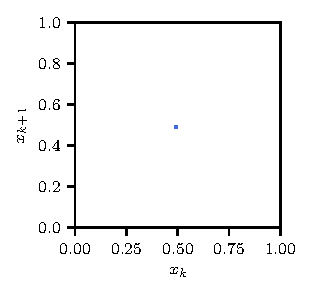
\includegraphics[width=.75\textwidth]{logistic_map_phase_plane_3}
	\end{minipage}

	\vspace{1cm}
\end{frame}

\begin{frame}[t, c]{Logistic map}{Cobweb and phase plane for $\mu = 2.28$}
	\begin{minipage}{.48\textwidth}
		\centering
		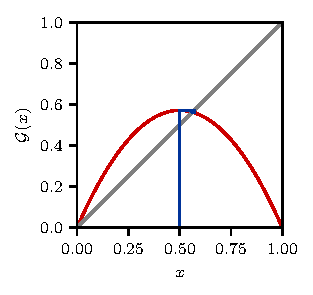
\includegraphics[width=.75\textwidth]{logistic_map_cobweb_plot_4}
	\end{minipage}%
	\begin{minipage}{.48\textwidth}
		\centering
		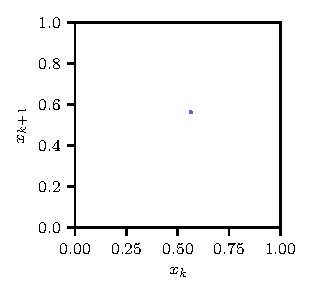
\includegraphics[width=.75\textwidth]{logistic_map_phase_plane_4}
	\end{minipage}

	\vspace{1cm}
\end{frame}

\begin{frame}[t, c]{Logistic map}{Cobweb and phase plane for $\mu = 2.61$}
	\begin{minipage}{.48\textwidth}
		\centering
		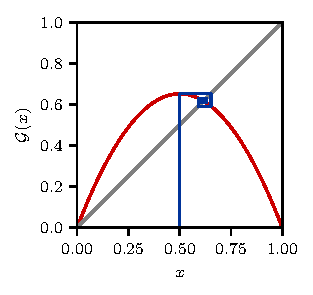
\includegraphics[width=.75\textwidth]{logistic_map_cobweb_plot_5}
	\end{minipage}%
	\begin{minipage}{.48\textwidth}
		\centering
		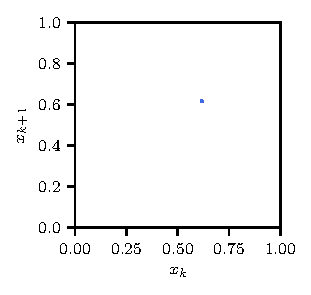
\includegraphics[width=.75\textwidth]{logistic_map_phase_plane_5}
	\end{minipage}

	\vspace{1cm}
\end{frame}

\begin{frame}[t, c]{Logistic map}{Cobweb and phase plane for $\mu = 2.93$}
	\begin{minipage}{.48\textwidth}
		\centering
		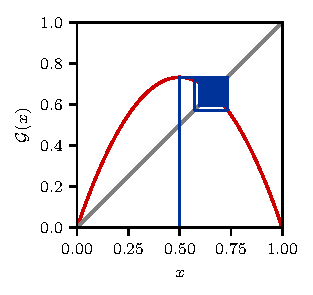
\includegraphics[width=.75\textwidth]{logistic_map_cobweb_plot_6}
	\end{minipage}%
	\begin{minipage}{.48\textwidth}
		\centering
		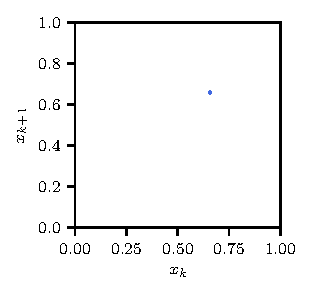
\includegraphics[width=.75\textwidth]{logistic_map_phase_plane_6}
	\end{minipage}

	\vspace{1cm}
\end{frame}

\begin{frame}[t, c]{Logistic map}{Cobweb and phase plane for $\mu = 3.25$}
	\begin{minipage}{.48\textwidth}
		\centering
		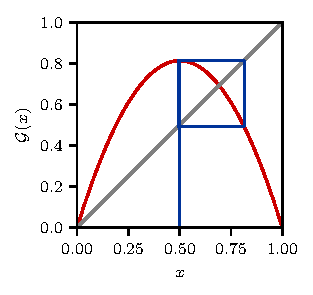
\includegraphics[width=.75\textwidth]{logistic_map_cobweb_plot_7}
	\end{minipage}%
	\begin{minipage}{.48\textwidth}
		\centering
		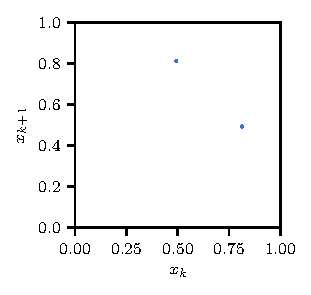
\includegraphics[width=.75\textwidth]{logistic_map_phase_plane_7}
	\end{minipage}

	\vspace{1cm}
\end{frame}

\begin{frame}[t, c]{Logistic map}{Cobweb and phase plane for $\mu = 3.57$}
	\begin{minipage}{.48\textwidth}
		\centering
		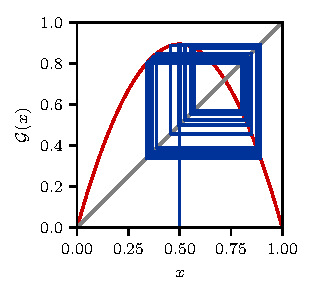
\includegraphics[width=.75\textwidth]{logistic_map_cobweb_plot_8}
	\end{minipage}%
	\begin{minipage}{.48\textwidth}
		\centering
		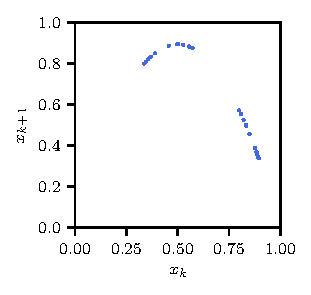
\includegraphics[width=.75\textwidth]{logistic_map_phase_plane_8}
	\end{minipage}

	\vspace{1cm}
\end{frame}

\begin{frame}[t, c]{Logistic map}{Cobweb and phase plane for $\mu = 3.9$}
	\begin{minipage}{.48\textwidth}
		\centering
		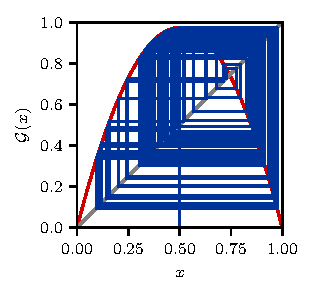
\includegraphics[width=.75\textwidth]{logistic_map_cobweb_plot_9}
	\end{minipage}%
	\begin{minipage}{.48\textwidth}
		\centering
		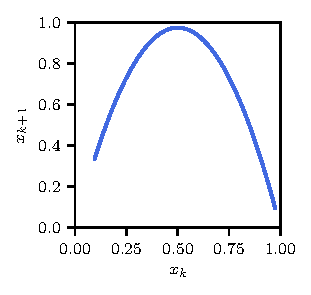
\includegraphics[width=.75\textwidth]{logistic_map_phase_plane_9}
	\end{minipage}

	\vspace{1cm}
\end{frame}

\begin{frame}[t, c]{Logistic map}{Bifurcation diagram}
	\centering
	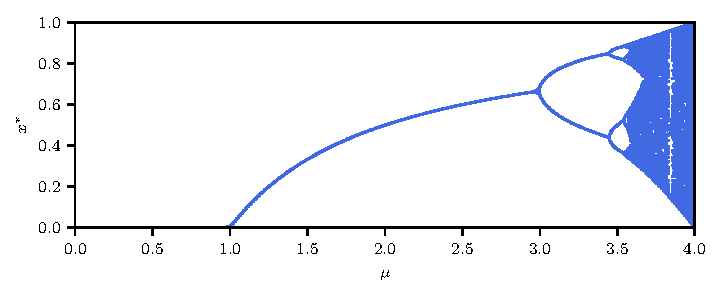
\includegraphics[width=.75\textwidth]{logistic_map_bifurcation_overview}

	\vspace{1cm}
\end{frame}

\begin{frame}[t, c]{Logistic map}{Bifurcation diagram}
	\centering
	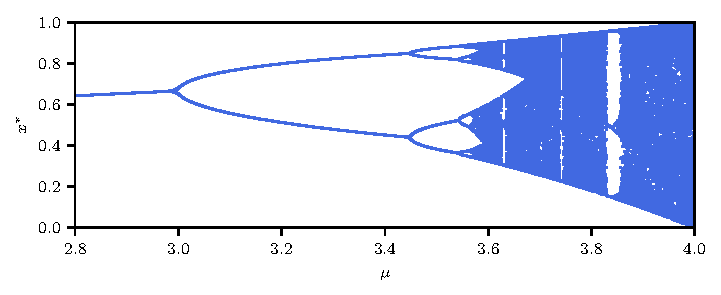
\includegraphics[width=.75\textwidth]{logistic_map_bifurcation_zoom_1}

	\vspace{1cm}
\end{frame}

\begin{frame}[t, c]{Logistic map}{Subharmonic cascade}
	\begin{itemize}
		\item At each bifurcation point, the period of the limit cycle doubles.
		\begin{itemize}
			\item[$\hookrightarrow$] $\mu_1 = 3 \to$ period 2.
			\item[$\hookrightarrow$] $\mu_2 = 3.449\cdots \to$ period 4.
			\item[$\hookrightarrow$] $\mu_3 = 3.54409\cdots \to$ period 8.
			\item[$\hookrightarrow$] $\mu_4 = 3.5644\cdots \to$ period 16.
			\item[$\hookrightarrow$] ...
		\end{itemize}

		\bigskip

		\item The sequence $\delta_i = \nicefrac{\mu_2 - \mu_1}{\mu_3 - \mu_2}$ converges to $\lim \limits_{i \to \infty} \delta_i = 4.669\cdots$.
	\end{itemize}

	\vspace{1cm}
\end{frame}

\begin{frame}[t, c]{}
	\centering
	\vspace{1cm}

	{\Large \textbf{R\"ossler system}}

	\bigskip

	{\textgre{\textbf{Period-doubling bifurcations in a continuous time system}}}

\end{frame}

\begin{frame}[t, c]{R\"ossler system}{A "simplified" Lorenz model}
	\begin{itemize}
		\item In 1976, Otto R\"ossler introduced this "simplified" version of Lorenz model
		\begin{equation}
			\begin{aligned}
				\dot{x} & = -y -z \\
				\dot{y} & = x + a y \\
				\dot{z} & = b + z(x-c).
			\end{aligned}
			\notag
		\end{equation}
		where we will assume $a=b=0.2$, while $c$ will be our control parameter.

		\bigskip

		\item Although its original goal was purely theoretical, this model has since then proven able to describe a certain class of chemical reactions.
	\end{itemize}

	\vspace{1cm}
\end{frame}

\begin{frame}[t, c]{R\"ossler system}{Period-doubling bifurcation in continuous-time systems}
	\centering
	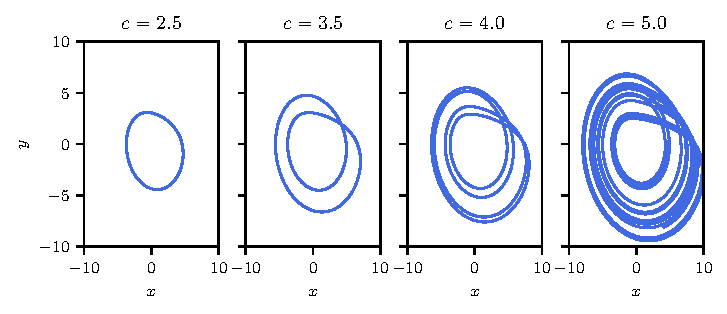
\includegraphics[width=.75\textwidth]{rossler_system_period_doubling}

	\vspace{1cm}
\end{frame}

\begin{frame}[t, c]{R\"ossler system}{Bifurcation diagram}
	\centering
	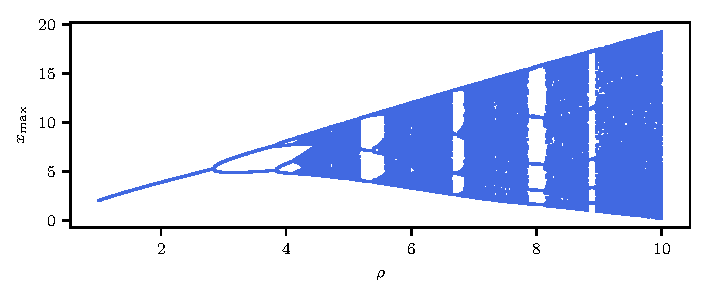
\includegraphics[width=.75\textwidth]{rossler_bifurcation_diagram}

	Bifurcation diagram of the R\"ossler system for $1 \leq c \leq 10$.

	\vspace{1cm}
\end{frame}

\begin{frame}[t, c]{R\"ossler system}{Bifurcation diagram}
	\centering
	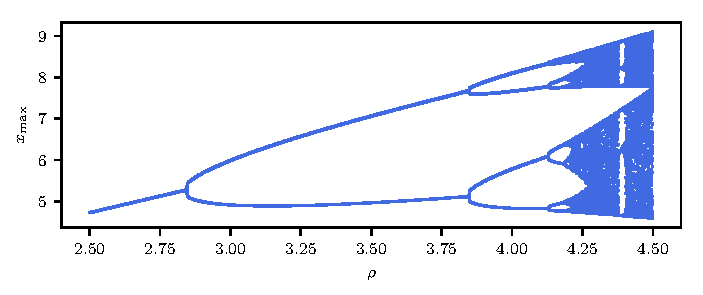
\includegraphics[width=.75\textwidth]{rossler_bifurcation_diagram_zoom}

	Bifurcation diagram of the R\"ossler system for $1 \leq c \leq 10$.

	\vspace{1cm}
\end{frame}

\begin{frame}[t, c]{R\"ossler system}{Bifurcation diagram}
	\centering
	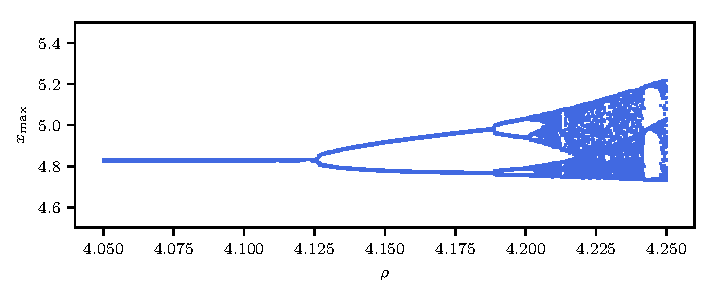
\includegraphics[width=.75\textwidth]{rossler_bifurcation_diagram_zoom_bis}

	Bifurcation diagram of the R\"ossler system for $1 \leq c \leq 10$.

	\vspace{1cm}
\end{frame}

\begin{frame}[t, c]{R\"ossler system}{Subharmonic cascade}
		\begin{itemize}
			\item As before, the period of the limit cycle doubles at each bifurcation point.
			\begin{itemize}
				\item[$\hookrightarrow$] $c_1 = ?? \to$ period 2.
				\item[$\hookrightarrow$] $c_2 = ?? \to$ period 4.
				\item[$\hookrightarrow$] $c_3 = ?? \to$ period 8.
				\item[$\hookrightarrow$] $c_4 = ?? \to$ period 16.
				\item[$\hookrightarrow$] ...
			\end{itemize}

			\bigskip

			\item Deep down, the transition to chaos for the R\"ossler system obeys the same law as the transition to chaos for the logistic map.
		\end{itemize}

		\vspace{1cm}
\end{frame}

\begin{frame}[t, c]{R\"ossler system}{From a 3D continuous-time system to a 1D discrete-time map}
	\centering
	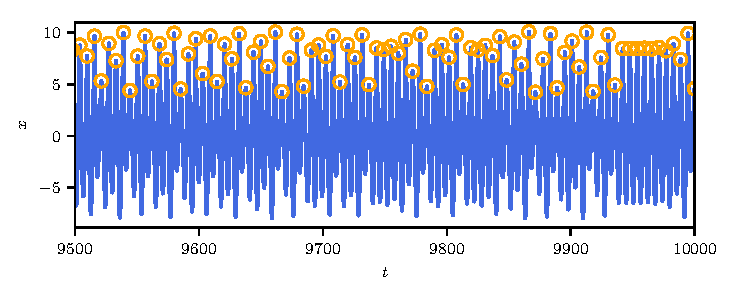
\includegraphics[width=.75\textwidth]{rossler_successive_maxima}

	Time series of $x(t)$ for $c=5$.

	\vspace{1cm}
\end{frame}

\begin{frame}[t, c]{R\"ossler system}{Lorenz map}
	\begin{minipage}{.48\textwidth}
		\begin{itemize}
			\item So-called \alert{\textbf{Lorenz map}} can be constructed using the R\"ossler system.

			\bigskip

			\item It is a (1D) \alert{\textbf{unimodal}} map very similar to the logistic map.

			\bigskip

			\item Such a 1D map emphasizes why the system exhibits a subharmonic cascade to chaos.
		\end{itemize}
	\end{minipage}%
	\hfill
	\begin{minipage}{.48\textwidth}
		\centering
		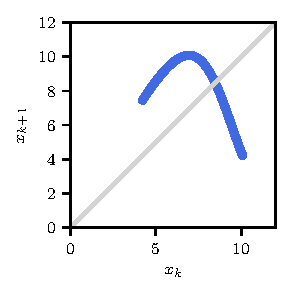
\includegraphics[width=.8\textwidth]{rossler_lorenz_map}
	\end{minipage}

	\vspace{1cm}
\end{frame}


\begin{frame}[t, c]{}
	\centering
	\vspace{1cm}

	{\Large \textbf{Self-similarity and Universality}}

	\bigskip

	{\textgre{\textbf{Feigenbaum and the Renormalization theory}}}

\end{frame}

\begin{frame}[t, c]{Renormalization theory}{A brief introduction}
	\begin{itemize}
		\item \alert{\textbf{Renormalization}} originated as a collection of techniques in quantum field theory, statistical mechanics of field and the theory of geometric structures.

		\bigskip

		\item During the 1970's, Feigenbaum borrowed ideas from renormalization theory to investigate the properties of the subharmonic cascade to chaos for 1D maps.
	\end{itemize}

	\vspace{1cm}
\end{frame}

\begin{frame}[t, c]{Renormalization theory}{Logistic map}
	\centering
	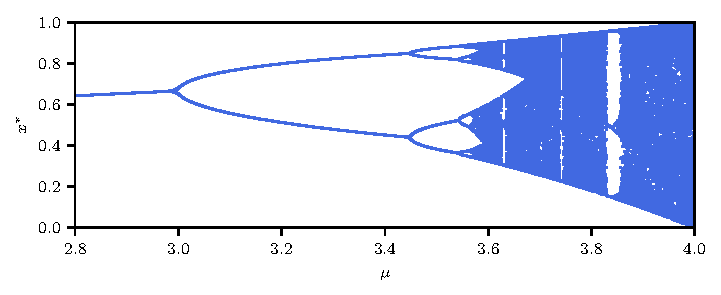
\includegraphics[width=.75\textwidth]{logistic_map_bifurcation_zoom_1}

	Bifurcation diagram of the logistic map $x_{k+1} = \mu x_k ( 1 - x_k)$.
	\vspace{1cm}
\end{frame}

\begin{frame}[t, c]{Renormalization theory}{Sine map}
	\centering
	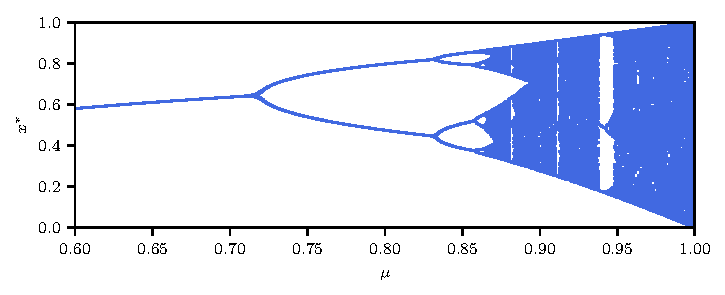
\includegraphics[width=.75\textwidth]{sine_map_bifurcation_diagram}

	Bifurcation diagram of the logistic map $x_{k+1} = \mu \sin \left( \pi x_k \right)$.
	\vspace{1cm}
\end{frame}

\begin{frame}[t, c]{Renormalization theory}{R\"ossler system}
	\centering
	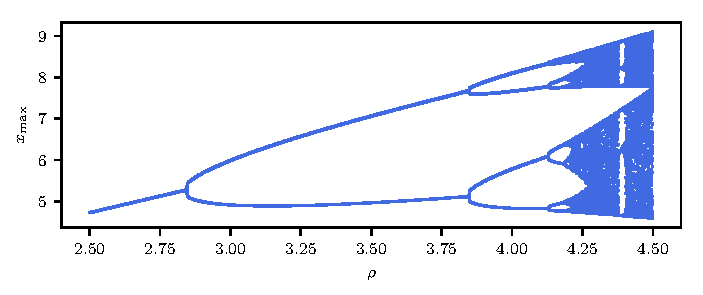
\includegraphics[width=.75\textwidth]{rossler_bifurcation_diagram_zoom}

	Bifurcation diagram of the R\"ossler system for $a=b=0.2$.

	\vspace{1cm}
\end{frame}

\begin{frame}[t, c]{Renormalization theory}{Unimodal maps}
	\begin{minipage}{.48\textwidth}
		\begin{itemize}
			\item All of the systems considered are \alert{\textbf{unimodal}} maps.

			\bigskip

			\item Their bifurcation diagrams all have the same geometric structure.
		\end{itemize}

		\vspace{1cm}
	\end{minipage}%
	\hfill
	\begin{minipage}{.48\textwidth}
		\centering
		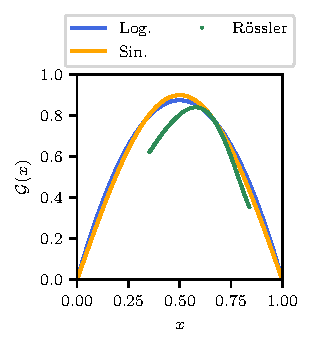
\includegraphics[width=.8\textwidth]{unimodal_maps}
	\end{minipage}

	\vspace{1cm}
\end{frame}

\begin{frame}[t, c]{Renormalization theory}{Pedagogical example}
	\begin{itemize}
		\item Let us consider the following normal form
		$$x_{k+1} = -(1 + \mu) x_k + x_k^2 + \cdots$$
		which undergoes a period doubling bifurcation as $\mu$ becomes positive.

		\bigskip

		\item The period-2 points, $p$ and $q$, are solution to
		\begin{equation}
			\begin{aligned}
				p & = (-1 + \mu)q + q^2 \\
				q & = (-1 + \mu)p + p^2,
			\end{aligned}
			\notag
		\end{equation}
		i.e.\ $f(q, \mu) = p$ and $f(p, \mu)= q$ with $f(x, \mu) = -(1 + \mu)x + x^2$.
	\end{itemize}
	\vspace{1cm}
\end{frame}

\begin{frame}[t, c]{Renormalization theory}{Pedagogical example}
	\begin{itemize}
		\item Points $p$ and $q$ are given by
		$p = \displaystyle \frac{\mu + \sqrt{\mu^2 + 4\mu}}{2}$ and $q = \displaystyle \frac{\mu - \sqrt{\mu^2 + 4\mu}}{2}$.

		\bigskip

		\item Shifting the origin to $p$, $p$ is now a fixed point of the map $f^2$.

		\bigskip

		\item Expand $p + \eta_{k+1} = f^2 (p + \eta_k)$ in powers of the deviation $\eta$.
	\end{itemize}

	\vspace{1cm}
\end{frame}

\begin{frame}[t, c]{Renormalization theory}{Pedagogical example}
	\begin{itemize}
		\item After proper rescaling, we obtain
		$$\tilde{x}_{k+1} = -(1 + \tilde{\mu}) \tilde{x}_k + \tilde{x}_k^2 + \cdots,$$
		where $\tilde{x} = (4 \mu + \mu^2 - 3\sqrt{\mu^2 + 4\mu}) \eta$ and $\tilde{\mu} = \mu^2 + 4\mu - 2$.

		\bigskip

		\item As $\tilde{\mu}$ becomes positive, this map undergoes a flip bifurcation.
		\begin{itemize}
			\item[$\hookrightarrow$] The 2-cycle of the original map loses its stability and a 4-cycle is created.
		\end{itemize}

		\bigskip

		\item This process can be repeated \emph{ad infinitum}!
	\end{itemize}

	\vspace{1cm}
\end{frame}

\begin{frame}[t, c]{Renormalization theory}{Pedagogical example}
	\begin{itemize}
		\item Repeating the procedure described previously, we obtain
		$$\mu_{k-1} = \mu_k^2 + 4\mu_k - 2$$
		or equivalently
		$$\mu_k = -2 + \sqrt{6 + \mu_k-1}.$$

		\bigskip

		\item It can be shown that $\lim \limits_{k \to \infty} \mu_k = \mu^*$, i.e.\ $\mu^*$ is a stable fixed point of the $\mu_k$-map which corresponds to the onset of chaos for our original map.
	\end{itemize}

	\vspace{1cm}
\end{frame}

\begin{frame}[t, c]{Renormalization theory}{Pedagogical example}
	\begin{enumerate}
		\item Compute the fixed point $\mu^*$ such that
		$$\mu^* = \left( \mu^* \right)^2 + 4\mu^* -2.$$

		\item Given $\mu^*$, compute the rescaling factor $\alpha$ given by
		$$\alpha = 4\mu + \mu^2 - 3\sqrt{\mu^2 + 4\mu}.$$

		\bigskip

		\item Given that $\delta = \nicefrac{\mu_{k-1} - \mu^*}{\mu_k - \mu^*} \simeq \nicefrac{\mathrm{d}\mu_{k-1}}{\mathrm{d}\mu_k}$, compute $\delta$.
	\end{enumerate}

	\vspace{1cm}
\end{frame}

\begin{frame}[t, c]{Renormalization theory}{Universal function}

\end{frame}

\begin{frame}[t, c]{Renormalization theory}{Universal function}
	\begin{itemize}
		\item At the onset of chaos, we have
		$$f(x) = \alpha f^2 \left( \displaystyle \frac{x}{\alpha} \right),$$
		along with the conditions $f(0) = 1$ and $f^{\prime}(0) = 0$.

		\bigskip

		\item This is a \emph{functional equation} for which we do not know (yet) a closed form solution.

		\bigskip

		\item Approximating $f(x)$ by a power series, one finally obtains $\alpha \simeq -2.509$.
		\begin{itemize}
			\item[$\hookrightarrow$] Although very simple, the $\alpha$ obtained in our example is only 10\% off from its true value!
		\end{itemize}
	\end{itemize}

	\vspace{1cm}
\end{frame}

\begin{frame}[t, c]{}
	\centering
	\vspace{1cm}

	{\Large \textbf{Lorenz system}}

	\bigskip

	{\textgre{\textbf{Period-doubling bifurcations in a continuous time system (again)}}}

\end{frame}

\begin{frame}[t, c]{Lorenz system}{Period-doubling bifurcations?}
	\centering
	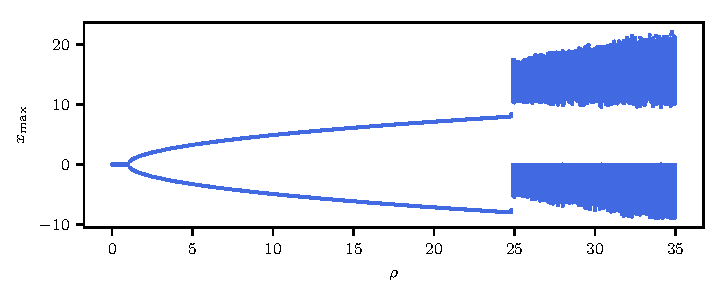
\includegraphics[width=.75\textwidth]{lorenz_bifurcation_diagram_1}

	Bifurcation diagram of the Lorenz system for $\sigma=10$ and $\beta = \nicefrac{8}{3}$.
	\vspace{1cm}
\end{frame}

\begin{frame}[t, c]{Lorenz system}{Period-doubling bifurcations?}
	\centering
	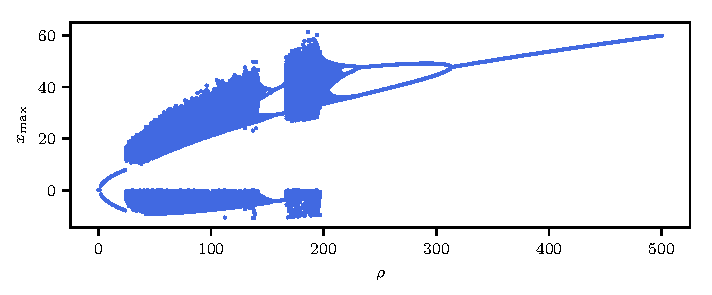
\includegraphics[width=.75\textwidth]{lorenz_bifurcation_diagram_2}

	Bifurcation diagram of the Lorenz system for $\sigma=10$ and $\beta = \nicefrac{8}{3}$.
	\vspace{1cm}
\end{frame}

\begin{frame}[t, c]{Lorenz system}{Subharmonic cascade to chaos}
	\begin{itemize}
		\item As $\rho$ decreases from 500, the Lorenz system exhibits a sequence of period-doubling bifurcations.
		\begin{itemize}
			\item[$\hookrightarrow$] $\rho_1 = 229.412 \cdots \to$ period 2.
			\item[$\hookrightarrow$] $\rho_2 = 218.2 \cdots \to$ period 4.
			\item[$\hookrightarrow$] $\rho_3 = 215.9665 \cdots \to$ period 8.
			\item[$\hookrightarrow$] $\rho_4 = 215.49231 \cdots \to$ period 16.
			\item[$\hookrightarrow$] $\rho_5 = 215.3908 \cdots \to$ period 32.
			\item[$\hookrightarrow$] $\rho_6 = 215.26440296 \cdots \to$ period 64.
			\item[$\hookrightarrow$] ...
		\end{itemize}

		\bigskip

		\item Just like before, the sequence $\rho_k$ (when appropriately normalized) obeys the same rule as for the logistic map (i.e.\ $\delta = 4.669 \cdots)$.

		\bigskip

		\item The onset of chaos through subharmonic cascade occurs at $\rho^* = 215.3631 \cdots$.
	\end{itemize}

	\vspace{1cm}
\end{frame}

\end{document}
